\documentclass[a4paper,%
11pt,%
DIV=12,
headsepline,%
headings=normal,
]{scrartcl}

\usepackage[utf8]{inputenc}
\usepackage[T1]{fontenc}
\usepackage[automark]{scrlayer-scrpage}
\usepackage{graphicx}
\usepackage{lmodern} 
\usepackage{url}
\usepackage{amsmath}
\usepackage{amssymb}
\usepackage{booktabs}
\usepackage{listings}

\usepackage{graphicx}
\graphicspath{ {../plots/} }

\lstset{
  basicstyle=\ttfamily\footnotesize,
  frame=single
}

\newcounter{curex}
\setcounter{curex}{0}
\newcommand{\exercise}[1]{\section*{Exercise #1}\setcounter{curex}{#1}}
\newcommand{\answer}[1]{\subsection*{Answer \arabic{curex}.#1}}

\newcommand\plotwidth{0.8\textwidth}
\newcommand\plotheight{0.48\textwidth}

\begin{document}

\noindent
\vspace*{1ex}
\begin{minipage}[t]{.45\linewidth}
\strut\vspace*{-\baselineskip}\newline

\includegraphics[height=.9cm]{./figs/Inf-Logo_black_en-eps-converted-to.pdf}

\includegraphics[height=.9cm]{./figs/par-logo}
\end{minipage}
\hfill
\begin{minipage}[t]{.5\linewidth}
\flushright{
Research Group for Parallel Computing\\%
Faculty of Informatics\\%
TU Wien}
\end{minipage}
\vspace*{1ex}

\hrule 

\vspace*{2ex}

\begin{center}
{\LARGE\textbf{Parallel Computing}}\\
{\large{}%
  2022S\\
  Übungsblatt 1\\
}
\end{center}

\hrule 
\vspace*{1ex}

\noindent
1: Jakob, Roithinger, 52009269\\
2: Elias, Pinter, 12023962\\
3: Kurdo-Jaroslav, Asinger, 01300351

\vspace*{1ex}
\hrule 

\exercise{1}

The source code snippets are just given here in case you would like to reuse them.
You can remove them in your solution if you want.
\begin{lstlisting}
void mv(int m, int n, double M[m][n], double V[n], double W[m])
{
  int i, j;

  for (i=0; i<m; i++) {
    W[i] = 0.0;
    for (j=0; j<n; j++) {
      W[i] += M[i][j]*V[j];
    }
  }
}
\end{lstlisting}

\answer{1}
\begin{lstlisting}
void mv(int m, int n, double M[m][n], double V[n], double W[m]){
  par(0<=i<m){
    W[i] = 0.0;
    for(int j = 0; j < n; j++){
      // summing into each cell in result vector 
      W[i] += M[i][j] * V[j];
    }
  }
}
\end{lstlisting}
requires the CREW PRAM model
\newpage
\answer{2}
\begin{lstlisting}
void mv(int m, int n, double M[m][n], double V[n], double W[m]) {
  
  par(0<=i<m, 0<=j<n){
    // doing actual multiplication in O(1) time steps (requires CREW PRAM)
    M[i][j] *= V[j];
  }

  // sum rows of Matrix in O(log(n)) time steps
  par(0<=i<m){
    int offset = 1;
    int betweenGap = 2;
    // sum of Matrix[i] in O(log(n)) time steps
    while(offset < n){
      // EREW summing, actually only n/betweenGap processors needed
      par(0<=j<n) {
        if(offset + j * betweenGap < n){
          M[i][j * betweenGap] += M[i][offset + j * betweenGap];
        }
      }
      offset *= 2;
      betweenGap *= 2;
    }
  }
  
  par(0<=i<n){
    // copying into result vector in O(1) time steps
    W[i] = M[i][0];
  }
}
\end{lstlisting}
requires the CREW PRAM model
\newpage
\answer{3}
\begin{lstlisting}
void mv(int m, int n, double M[m][n], double V[n], double W[m]){
  double C[m][n];
  par(0<=j<n){
    // copying vector into intermediate matrix in O(1) time steps
    C[0][j] = V[j];
  }

  // making m copies of V in O(log(n)) time steps
  offset = 1;
  // O(log(n)) loops
  while(offset < m){
    // duplicating existing vectors in O(1)
    par(0<=i<m){
      if(i + offset < m){
        par(0<=j<n){
          C[i + offset][j] = C[i][j]
        }
      }
    }
    offset *= 2;
  }

  par(0<=i<m, 0<=j<n){
    // calculating summands in O(1) time steps
    M[i][j] = M[i][j] * C[i][j];
  }
    
  par(0<=i<m){
    int offset = 1;
    int betweenGap = 2;
    // sum row [i] of Matrix in O(log(n)) time steps
    while(offset < n){
      // EREW summing, actually only n/betweenGap processors needed
      par(0<=j<n) {
        if(offset + j * betweenGap < n){
          M[i][j * betweenGap] += M[i][offset + j * betweenGap];
        }
      }
      offset *= 2;
      betweenGap *= 2;
    }
  }

  par(0<=i<n){
    // copying into result vector in O(1) time steps
    W[i] = M[i][0];
  }
}
\end{lstlisting}
requires the EREW PRAM model

\exercise{2}

\begin{lstlisting}
for (i=0; i<n; i++) {
  int count = 0;
  for (j=0; j<i; j++) {
    if (a[j]<=a[i]) count++;
  }
  j++;
  for (; j<n; j++) {
    if (a[j]<a[i]) count++;
  }
  b[count] = a[i];
}
for (i=0; i<n; i++) a[i] = b[i];
\end{lstlisting}

\answer{1}
The program sorts a given array of integers in ascending order. A comparison with "$a \leq \ b$" has to be done in for all b that come before a, so that the program also sorts array with duplicates. If $<=$ is not used for all b that come before a, all duplicates will end up at the same index in the result, causing ``gaps'' (some array entries will have undefined/default initialization value). Using $<=$ also guarantees stability, meaning that the relative order of equal elements in the input will be sustained in the output.

\answer{2}
The asymptotic sequential work of the given algorithm is $O(n^{2})$. The outer loop is executed n times. Within this loop, there are two nested loops which have a total of $n-1 (= O(n))$ iterations (j run from 0 to i, and then from i + 1 to n), each with $O(1)$ work. After the first (outer) loop, there is another loop which is executed n times, with $O(1)$ work per iteration. This concludes to the work of $O(n^{2})$. Here is the code once again, with explanation regarding work in the comments:

% TODO REVIEW dependent on i is not canonical though?
% TODO REVIEW not necessary?
\begin{lstlisting}
for (i=0; i<n; i++) {            // canonical loop dependent on n
  int count = 0;                 // constant work
  for (j=0; j<i; j++) {          // canonical loop dependent on i
    if (a[j]<=a[i]) count++;     // constant work
  }
  j++;                           // constant work
  for (; j<n; j++) {             // linear loop dependent on the i-loop and n
    if (a[j]<a[i]) count++;      // constant work
  }
  b[count] = a[i];               // constant work
}
for (i=0; i<n; i++)              // canonical loop dependent on n
  a[i] = b[i];                   // constant work
\end{lstlisting}

% TODO REVIEW exact iterations?
\begin{math}n*(1 + n*(1) + 1 + n*(1) + 1) + n*(1) =\end{math}\\
\begin{math}n*(n + 3) + n =\end{math}\\
\begin{math}n^2 + 4n\end{math}\\
\begin{math}n^2 + 4n \in O(n^2)\end{math}\\
This is a very simplified calculation. The j-loop's workload rises as the i-loop's workload shrinks. Generally, within one outer-loop iteration, the sum of the iterations of the first and second j-loop together is n. However, it does not make in difference for the big O notation.

\answer{3}
\begin{lstlisting}
#include <omp.h>
// assume a, b initialized arrays, each with a capacity of n integers
#pragma omp parallel default(none) shared(a, b) firstprivate(n)
{
  int i;
  #pragma omp for
  for (i = 0; i < n; i++) {
   int count = 0;
   int j;
   for (j = 0; j < i; j++) {
    if (a[j] <= a[i]) count++;
   }
    j++;
   for (; j < n; j++) {
    if (a[j] < a[i]) count++;
   }
   b[count] = a[i];
  }
  // implicit barrier
  #pragma omp for
  for (i = 0; i < n; i++) {
   a[i] = b[i];
 }
}
\end{lstlisting}

\answer{4}
The outer loop is embarrassingly parallel, because the iterations are independent of each other. Therefore, the speedup is linear (compared to the sequential execution of this algorithm). So assuming $n \geq p$ the runtime will be in:\\
\begin{math}O(\frac{n^2}{p})\end{math}\\

\answer{5}
Relative speedup will be linear as long as $p \leq n$.\\

\begin{math}SRel_{p}(n)=\frac{T_{par}(1,n)}{T_{par}(p,n)} = \frac{n^2}{n^2/p} = p \end{math}\\
The absolute speedup has to be compared with the best known sequantial algorithm for this problem (sorting). Mergesort is on of these, running in \begin{math}O(n \cdot log(n))\end{math}. The absulote speed-up is not linear.\\

\begin{math}S_{p}(n)=\frac{T_{seq}(n)}{T_{par}(p,n)} = \frac{n \cdot log(n)}{n^2/p} = \frac{log(n) \cdot p}{n} \end{math}\\



\exercise{3}
\begin{lstlisting}
# pragma omp parallel for schedule ( runtime )
for (i = 0; i < n ; i++) {
  a[i] = omp_get_thread_num();
  t[omp_get_thread_num()]++;
}
\end{lstlisting}
\answer{1}
a[i] tracks which thread executed iteration \emph{i} in the for loop.
t[i] tracks how many iterations were executed by thread \emph{i}.

\answer{2}


\begin{tabular}{rrrrrrrrrrrrrrrrrrrr}
  \toprule
 case /  $i$ & 0 & 1 & 2 & 3 & 4 & 5 & 6 & 7 & 8 & 9 & 10 & 11 & 12 & 13 & 14 & 15 & 16 & 17 & 18  \\
  \midrule
\texttt{static}     & 0 & 0 & 0 & 1 & 1 & 1 & 2 & 2 & 2 & 3 & 3 & 3 & 4 & 4 & 4 & 5 & 5 & 5 & 0 \\
\texttt{static,2}   & 0 & 0 & 1 & 1 & 2 & 2 & 3 & 3 & 4 & 4 & 5 & 5 & 0 & 0 & 1 & 1 & 2 & 2 & 3 \\
\texttt{static,5}   & 0 & 0 & 0 & 0 & 0 & 1 & 1 & 1 & 1 & 1 & 2 & 2 & 2 & 2 & 2 & 3 & 3 & 3 & 3 \\
\texttt{static,6}   & 0 & 0 & 0 & 0 & 0 & 0 & 1 & 1 & 1 & 1 & 1 & 1 & 2 & 2 & 2 & 2 & 2 & 2 & 3 \\ 
\texttt{dynamic,1}  & 0 & 1 & 2 & 3 & 4 & 5 & 0 & 1 & 2 & 3 & 4 & 5 & 0 & 1 & 2 & 3 & 4 & 5 & 0 \\
\texttt{dynamic,2}  & 0 & 0 & 1 & 1 & 2 & 2 & 3 & 3 & 4 & 4 & 5 & 5 & 0 & 0 & 1 & 1 & 2 & 2 & 3 \\
  \texttt{guided,3} & 0 & 0 & 0 & 1 & 1 & 1 & 2 & 2 & 2 & 3 & 3 & 3 & 4 & 4 & 4 & 5 & 5 & 5 & 0 \\
  \bottomrule
\end{tabular}\\

\begin{tabular}{rrrrrrr}
  \toprule
case / $t$             & $t[0]$ & $t[1]$ & $t[2]$ & $t[3]$ & $t[4]$ & $t[5]$ \\  
  \midrule
\texttt{static}    & 4 & 3 & 3 & 3 & 3 & 3 \\
\texttt{static,2}  & 4 & 4 & 4 & 3 & 2 & 2 \\
\texttt{static,5}  & 5 & 5 & 5 & 4 & 0 & 0 \\
\texttt{static,6}  & 6 & 6 & 6 & 1 & 0 & 0 \\
\texttt{dynamic,1} & 4 & 3 & 3 & 3 & 3 & 3 \\
\texttt{dynamic,2} & 4 & 4 & 4 & 3 & 2 & 2 \\
\texttt{guided,3}  & 4 & 3 & 3 & 3 & 3 & 3 \\
    \bottomrule
\end{tabular}

\answer{3}
False sharing is a possible performance issue:
Multiple threads (on different cores) may want to access t (at different indexes i and j) at close points in time. If two indexes i, j are close enough and positioned in a way that t[i] and t[j] are on the same cache line, and t[i] t[j] are accessed by different threads, they will be ``falsely shared'' and cache coherency activity will occur, which impacts performance considerably. 

\exercise{4}

\begin{lstlisting}
i = 0; j = 0; k = 0; 
while (i<n&&j<m) {
   C[k++] = (A[i]<=B[j]) ? A[i++] : B[j++]; 
}
while (i<n) C[k++] = A[i++]; 
while (j<m) C[k++] = B[j++];
\end{lstlisting}

\answer{1}
Assuming i, j, k are in registers. \\
Example for a best case input for A and B:
A = [0,0,0,0 ...] 
B = [1,1,1,1 ...] \\
This way A[0] will be fetched with a cache miss, then B[0] will be fetched with a cache miss (stored in a register afterwards), overwriting the cache line with A[0] stored. Then A[0] will be inserted at C[0].
Then A[1] will be fetched, resulting in a cache miss, however the rest of A will be fetched and inserted into C, resulting in a cache miss every 16 elements. \\
Then all of B will be inserted into C, also resulting in a cache miss every 16 elements. \\
Total cache misses: 2 + 2n/16 = 2 + n/8, \textbf{cache miss rate:} 1/16

\answer{2}
Example for a worst case input for A and B:
A = [1,2,3,4 ...] 
B = [1,2,3,4 ...] \\
If A and B contain the same values that are also strictly increasing, alternating at every iteration first A[i] <= B[j] will hold, and in the next A[i] > B[j]. At every iteration a new element has to be fetched from memory, but a miss will always occur, as the cache line will contain elements from A[i] when an element from B[j] is needed, and vice versa.  
Total cache misses: 2n, \textbf{cache miss rate:} 1.0

\exercise{5}

\answer{1}
A parallel section is opened, with to omp for constructs. In the first for-construct every element in \emph{A} is ranked in the array \emph{B} and inserted accordingly in \emph{C}. It is marked as no wait, as there are no data conflicts. In the second for-construct every element in \emph{B} is ranked in the array \emph{A} and then inserted accordingly in \emph{C}. Ranking is done sequentially by binary search in O(log(n)), inserting into \emph{C} is done for n + m elements in parallel, in O(1) time. Therefore the runtime is $ O((n + m)/p \cdot log(n))$.


\answer{2}

% TODO make look nice, use speed up

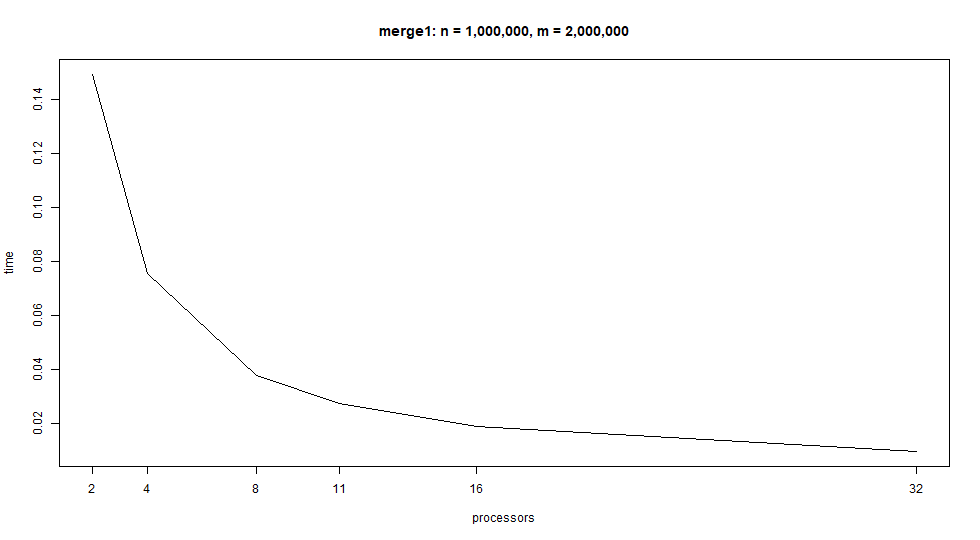
\includegraphics[width=\plotwidth, height=\plotheight]{plot_merge1_run1_1000000_2000000.png}\\
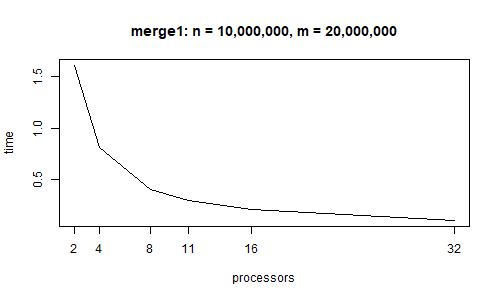
\includegraphics[width=\plotwidth, height=\plotheight]{plot_merge1_run1_10000000_20000000.png}\\
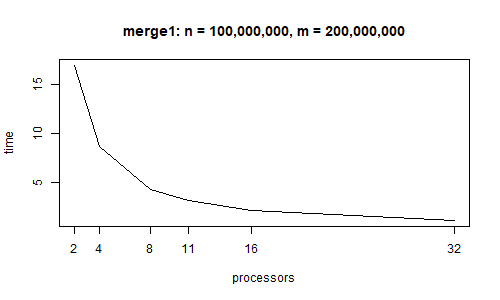
\includegraphics[width=\plotwidth, height=\plotheight]{plot_merge1_run1_100000000_200000000.png}\\



\answer{3}
To make the merge stable, nothing has to be done to preserve relative order of equal elements in A as well as B in C.
To make sure equal elements of A come before equal elements of B: \\
Rewrite rank algorithm:\\
rank{\_}for{\_}A(a, B, m) returns a j such that B[j] < a <= B[j + 1] \\
and another algorithm: \\
rank{\_}for{\_}B(b, A, n) returns an i such that A[i] <= b < A[i + 1]


\exercise{6}

\begin{lstlisting}
void merge_corank(double A[], int n, double B[], int m, double C[])
{
  int t; // number of blocks (threads)
  int i;
  
  int coj[t+1];
  int cok[t+1];
  
  for (i=0; i<t; i++) {
    corank(i*(n+m)/t,A,n,&coj[i],B,m,&cok[i]);
  }
  coj[t] = n;
  cok[t] = m;
  
  for (i=0; i<t; i++) {
    merge(&A[coj[i]],coj[i+1]-coj[i],
    &B[cok[i]],cok[i+1]-cok[i],
    &C[i*(n+m)/t]);
  }
}
\end{lstlisting}

\answer{1}
The asymptotic complexity can be calculated as follows:\\
\\
$O(t * log(n+m) + t * \frac{n+m}{t}) = O(n+m+t*log(n+m))$
\answer{2}

\answer{3}

\answer{4}
Currently in the program there is an implicit barrier required after calculating the co-ranks:\\
  \begin{lstlisting}
  #pragma omp for SCHEDULE_STRATEGY
  for (i = 0; i < t; i++) {
      corank(i * (n + m) / t, A, n, &coj[i], B, m, &cok[i]);
  }
  \end{lstlisting}
If we calculate the co-ranks twicr per block as follows we can get rid of this synchronisation:
  \begin{lstlisting}
  if(omp_get_thread_num != t-1){
    corank(omp_get_thread_num * (n + m) / t, A, n, &coj[i], B, m, &cok[i]);
    corank((omp_get_thread_num + 1) * (n + m) / t, A, n, &coj[i], B, m, &cok[i]);
  }
  seq_merge1(&A[coj[i]], coj[omp_get_thread_num + 1] - coj[omp_get_thread_num], &B[cok[i]], cok[omp_get_thread_num + 1] - cok[omp_get_thread_num], &C[omp_get_thread_num * (n + m) / t]);
  \end{lstlisting}

\exercise{7}

\begin{lstlisting}
void merge_divconq(double A[], int n, double B[], int m, double C[])
{
  int i;

  if (n==0) { // task parallelize for large n
    for (i=0; i<m; i++) C[i] = B[i];
  } else if (m==0) { // task parallelize for large m
    for (i=0; i<n; i++) C[i] = A[i];
  } else if (n+m<CUTOFF) {
    merge(A,n,B,m,C); // sequential merge for small problems
  } else {
    int r = n/2;
    int s = rank(A[r],B,m);
    C[r+s] = A[r];
    merge_divconq(A,r,B,s,C);
    merge_divconq(&A[r+1],n-r-1,&B[s],m-s,&C[r+s+1]);
  }
}
\end{lstlisting}

\answer{1}

\answer{2}
Testing empirically showed that a very good cut-off value can be calculated with the following function $cutoff(n,m,t) = \frac{n \cdot m}{p}$.
where n and m are the lengths of the arrays A and B before performing any recursion steps

\answer{3}

\exercise{8}

\answer{1}

\answer{2}

\answer{3}

\exercise{9}

\answer{1}

\answer{2}

\answer{3}


\end{document}
